\section{Opgeleverde Producten en Diensten}

\subsection{Solver}

\subsubsection*{Chaining}
Het chaining algoritme, dat is ge\"introduceerd in paragraaf \ref{subsubsec:chainingoplossing}, is ge\"implementeerd, waarbij een keuze is tussen drie verschillende methoden voor het selecteren van een chain, namelijk:
\begin{itemize}
\item Selecteer de eerst gevonden geschikte chain.
\item Selecteer een willekeurige geschikte.
\item Gebruik de heuristiek beschreven in \ref{subsubsec:chainingoplossing}.
\end{itemize}

\subsection*{Linear Programming}
Om voor elke taak een flexibiliteitsinterval te vinden, moet er, zoals beschreven in paragraaf \ref{subsec:probleemoplossing}, een LP-probleem opgelost worden. Om dit gemakkelijk te kunnen doen, wordt de CLP\footnote{\href{https://projects.coin-or.org/Clp}{projects.coin-or.org/Clp}} (COIN-OR Linear Programming) library gebruikt. Deze library verwacht als input een stelsel lineaire vergelijkingen en een variabele om te optimaliseren, en geeft als output de geoptimaliseerde waarde en voor elke variabele de toekenning.

Hoe het toevoegen van rows gebeurt enzo...

\subsection{Interface}
De grootste veranderingen aan de interface zijn het weergeven van de chains en de flexibiliteitsintervallen. Deze worden als volgt in de interface weergegeven:

\begin{figure}
\label{fig:GUIfinal}
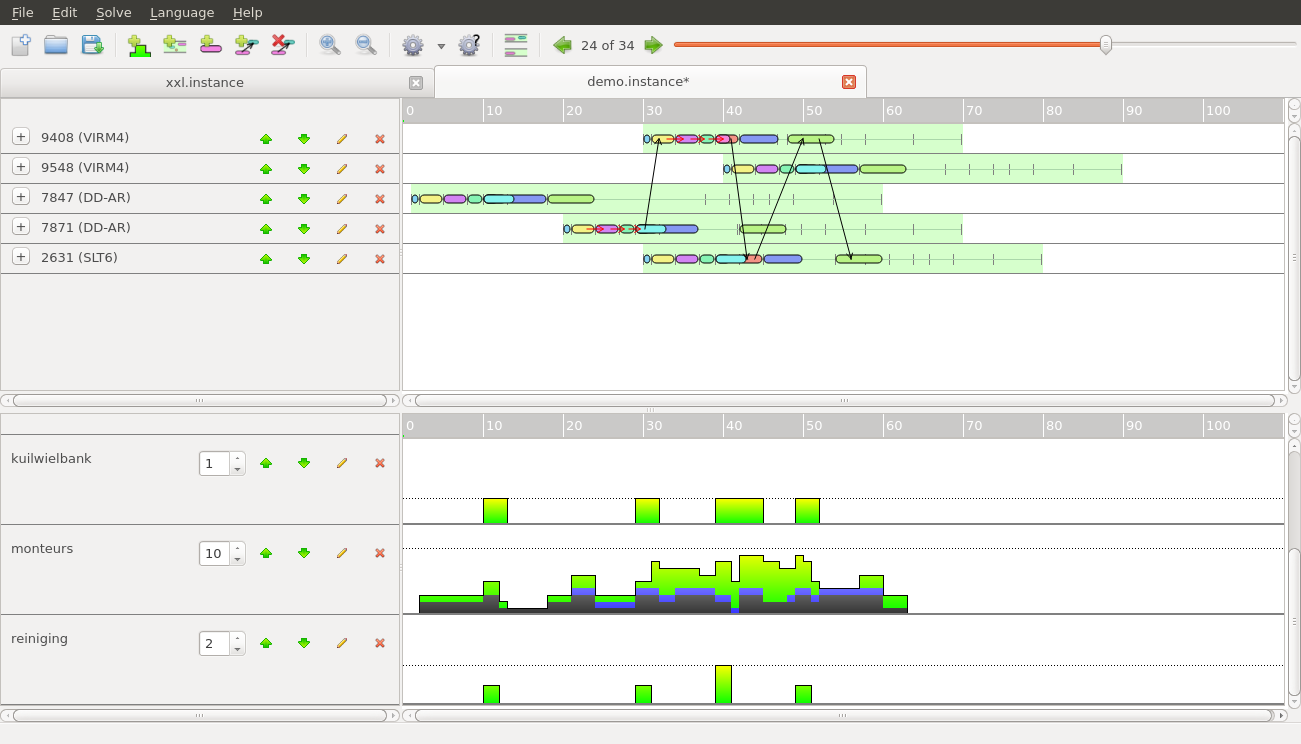
\includegraphics[width=\textwidth]{../images/GUIfinal.png}
\caption{De grafische gebruikersinterface.}
\end{figure}

In het bovenstaande figuur is in de rechterbovenhoek een schuifbalk te zien, waarmee verschillende stappen van het proces van de solver laten zien kunnen worden in de interface. Naar zo'n stap, waarin de toestand van alle activiteiten opgeslagen in, zal vanaf nu gerefereerd worden als een frame. De volgende frames worden toegevoegd na het uitvoeren van een solver:
\begin{itemize}
\item Een frame met de begintoestand van de instantie.
\item Voor elke voorrangsrelatie die tijdens het ESTA$^+$ algoritme toegevoegd wordt, een nieuw frame met daarop alleen de nieuwe voorrangsrelatie en eventuele veranderingen in starttijden van de activiteiten.
\item Een frame zonder voorrangsrelaties, waarin geen resource conflicten meer aanwezig zijn. Op dit moment worden alle eerder toegevoegde voorrangsrelaties verwijderd.
\item Voor elke resource een frame waarop alle bij deze resource horende chains getoond worden. Vervolgens een apart frame voor elke chain, die elk bij 1 resource unit hoort. Voor lege chains zal geen frame toegevoegd worden, maar voor chains met maar 1 activiteit wel.
\item Tenslotte een frame waarin voor elke activiteit in het blauw een flexibiliteitsinterval te zien is. Activiteiten worden ook verplaatst, zodat ze zich volledig in het blauwe interval bevinden.
\end{itemize}
Als een solver geen chains en/of flexibiliteitsintervallen berekent, zullen voor deze stappen geen frames worden toegevoegd en zullen alleen de frames van het ESTA$^+$-algoritme getoond worden.

In het frame dat in Figuur \ref{fig:GUIfinal} zichtbaar is, wordt een chain van activiteiten, behorende bij de resource 'monteurs', in het bovenste deelvenster getoond. Hierin zijn de rode pijlen voorrangsrelaties die al in de instantie aanwezig waren en zijn de zwarte pijlen later toegevoegd tijdens het oplossen van de instantie.

%Zodra de solver klaar is met het vinden van een oplossing voor de huidige instantie, wordt deze oplossing als output gegeven en geparsed door de planner. Vervolgens worden in de interface voor elke resource eerst een frame met alle chains van deze resource en toegevoegd en daarna voor al deze chains een aparte frame.

- weergeven van flexibiliteitsintervals
- verschuiven van taken/resources

Waar eerst instanties gesloten konden worden met een grote rode knop in de menubalk, is er nu op elke tab van een instantie een kruisje geplaatst, waarmee de instantie gesloten kan worden. Dit ontwerp ziet er intu\"itief uit en wordt ook gebruikt door bijvoorbeeld de veelgebruikt browser Google Chrome.

Er zijn ook sneltoetsen toegevoegd voor het in- en uitzoomen en voor het horizontaal scrollen. Er kan in- en uitgezoomd worden door de ctrl-toets ingedrukt te houden en het scrollwiel van de muis  te bewegen. Horizontaal scrollen kan in het venster waarin de muis zich op dat moment bevindt door de shift-toets ingedrukt te houden en het scrollwiel van de muis te bewegen. Deze sneltoetsen zijn ingesteld zodat de gebruiker makkelijker door een probleeminstantie kan navigeren, zonder daarvoor steeds zijn muis naar de menubalk te hoeven verplaatsen.

\subsection{Port naar Windows 7}
Om de toegankelijkheid van de applicatie te vergroten, is ervoor gezorgd dat deze ook op het besturingssysteem Windows 7 werkt. Hierbij is het ook nog steeds mogelijk om deze op Unix-based systemen te draaien, zoals Ubuntu. Alle functies van het programma moeten dus zowel op Windows 7 als op Ubuntu correct werken.

\subsection{Upgrade naar Qt 5.2}
De bestaande applicatie was ontwikkeld in versie 4.8 van het Qt framework, maar om de applicatie zo up-to-date mogelijk te houden, is deze geport naar Qt versie 5.2. Hierdoor hoeft een eventuele groep die de applicatie verder gaat ontwikkelen, niet met een oude versie van het Qt framework te werken. Deze upgrade betekent echter ook dat de applicatie niet meer werkt met Qt 4, maar alleen met versie 5.